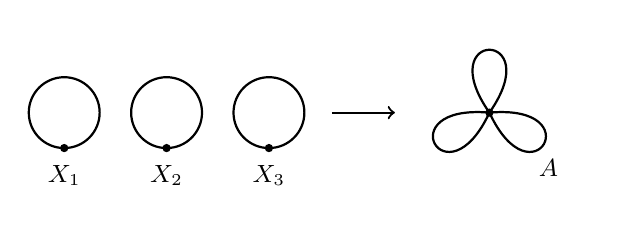
\begin{tikzpicture}[line width=0.8pt, every node/.style={font=\small}]
  \foreach \x/\l in {0/1, 1.3/2, 2.6/3} {
    \draw (\x,0.45) circle (0.45);
    \fill (\x,0) circle (1.5pt);
    \node at (\x,-0.35) {$X_{\l}$};
  }
  \draw[->] (3.4,0.45) -- (4.2,0.45);
  \begin{scope}[shift={(5.4,0.45)}]
    \foreach \a in {90, 210, 330} {
      \draw (0,0) .. controls ++(\a-35:1.3) and ++(\a+35:1.3) .. (0,0);
    }
    \fill (0,0) circle (1.5pt);
    \node at (0.75,-0.7) {$A$};
  \end{scope}
\end{tikzpicture}
